\chapter{The Latte Framework}

\section{Introduction}
The Latte framework forms the software basis for almost all of the reconstruction algorithms described in this thesis. It acts as both a set of utilities and a unifying central control mechanism. This chapter discusses several of the algorithms provided, ending with an overview of the control structures of the Latte framework itself. Some components of Latte form a significant contribution to the work in this thesis, and are discussed separately in subsequent chapters.

\section{Nearest Neighbour Search using \acs{KDTree}}\label{sec:latte_kdtree}
The \ac{KDTree} is a data structure for partitioning a $k$-dimensional space by representing the points as nodes in a binary tree. Using a \ac{KDTree} it is possible to perform nearest-neighbour search in $O(\log N)$ time\citep{Bentley1975},\footnote{$N$ is the number of data points to be partitioned. The KDTree itself is built in $O(kN\log N)$ time.} compared with the brute-force search complexity of $O(N^2)$. An introductory tutorial on \aclp{KDTree} appears in \citep{Moore1991}. The \ac{KDTree} is not a clustering algorithm, but its rapid near-neighbour search forms a central part of several clustering algorithms, as well as being used for the charge weighting procedure (see chapter \ref{sec:cellularautomaton_charge_weighting}) and the cell generation (chapter \ref{sec:cellularautomaton_cell_generation}) stage of the \acl{CA} track reconstruction procedure.

The implementation currently used is that of the \emph{SciPy}\citep{SciPy} library of Python code for scientific computing.

\section{Charge Weighting}\label{sec:cellularautomaton_charge_weighting}
Data from a \ac{LAr TPC} is assumed to be in the form of $(x, y, z)$ voxels with an associated charge deposit $Q$. The voxel shape is determined entirely by the readout mechanism; a 2D readout plane determines the $xy$ resolution while the readout sampling rate determines the $z$ resolution as expected for a \ac{TPC}. This structure is retained in the Geant4 simulation through the use of cubic voxels with a side length of $1\mm$. In order to transform this data into a representation more closely resembling the true passage of ionising radiation through the detector, a charge weighting procedure is applied. This procedure adjusts the spatial coordinates of each charge deposit (voxel) by taking the charge-weighted average of the spatial coordinates of all hits within a sphere of some radius (default: $2\mm$) centered on that voxel:

\begin{equation}\label{eqn:charge_weighted_avg_position}
	\vec{x}^\prime = \frac{\displaystyle \sum_i \vec{x}_i Q_i}{\displaystyle \sum_i Q_i}
\end{equation}

The neighbouring hits are discovered using the \ac{KDTree} algorithm described in section \ref{sec:latte_kdtree}.

Charge weighting\footnote{This is not, strictly speaking, the usual definition of charge weighting, in which a set of hits is reduced to a smaller set of charge-weighted hits, but more of a smoothing process to reduce the geometric effects of the readout system. Hits are retained here primarily to facilitate accessing truth information.} in this way moves the position of each charge deposit closer to the local charge cloud, bringing track-like charge deposits closer to a straight line (see figure \ref{fig:ca_charge_weighting}). For each point, the sum is taken over the unweighted positions of neighbours and a new dataset is generated, containing the weighted positions. This results in a stable, deterministic output.

\begin{figure}
\centering
\subfigure[Hits as central points of voxels]{
	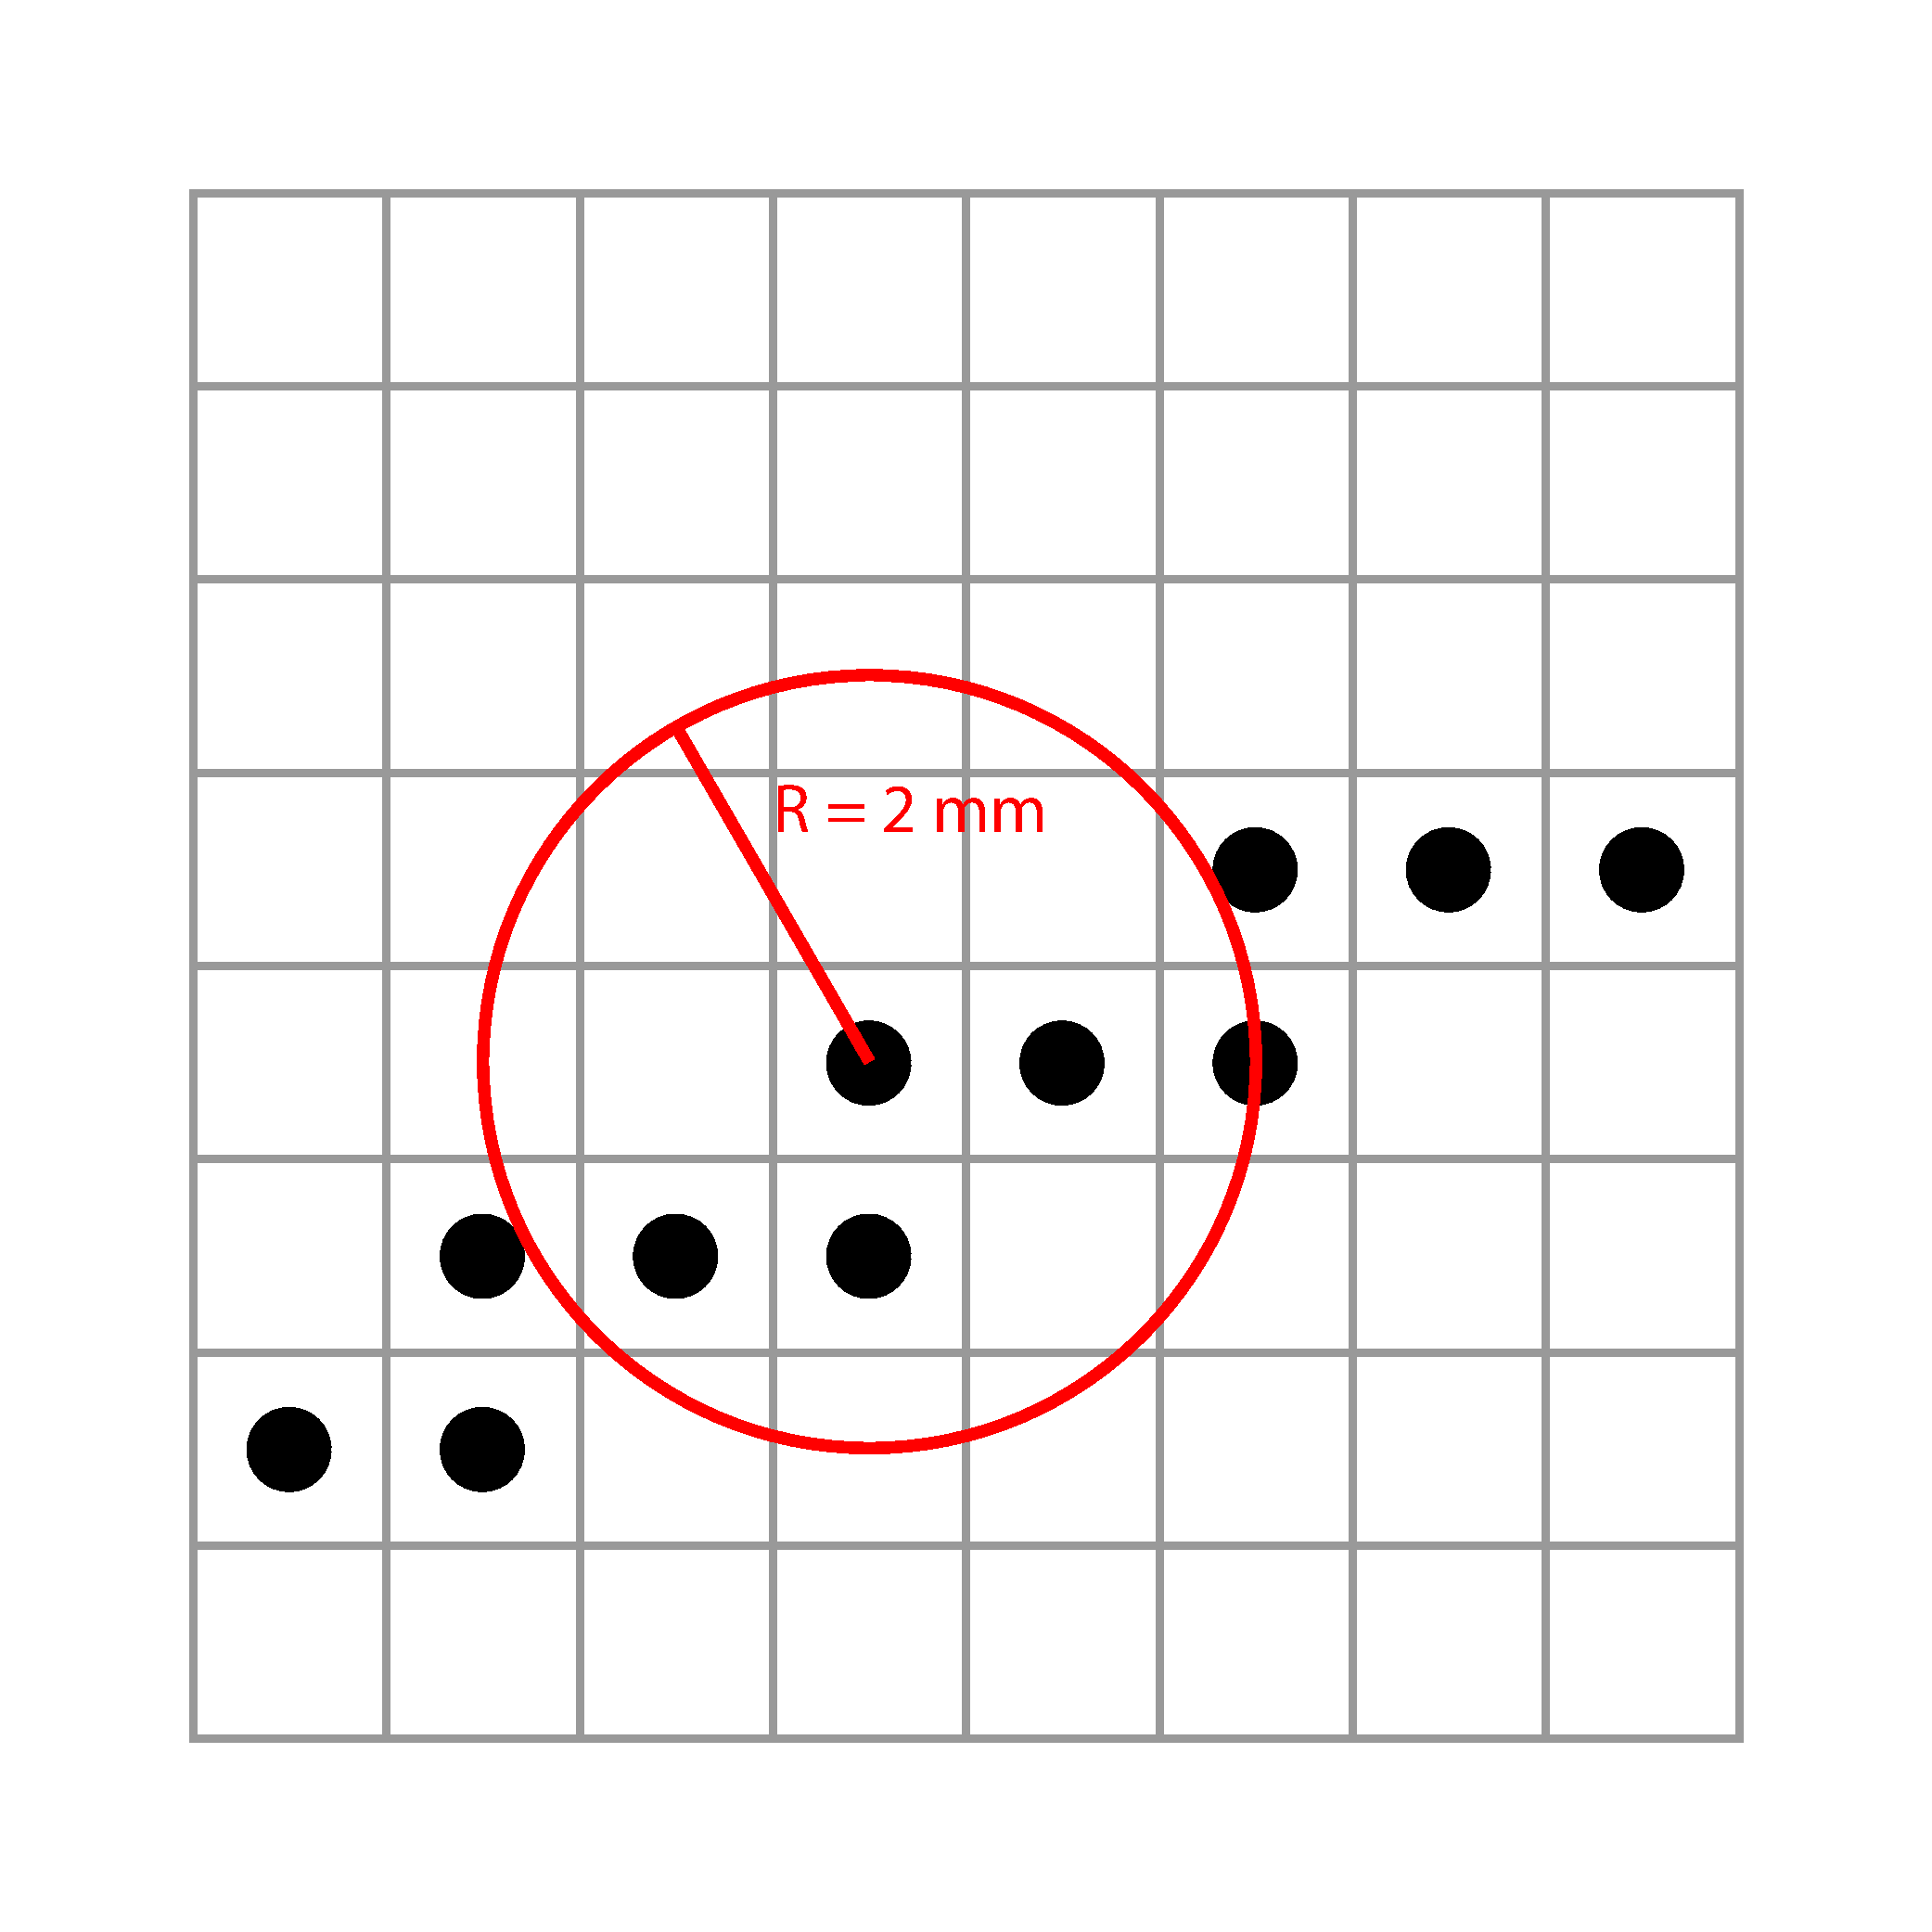
\includegraphics[width=0.4\textwidth]{chapters/cellularautomaton_images/ChargeWeighting1}
	\label{fig:ca_charge_weighting_1}
}
\subfigure[Hits shifted from voxel centres]{
	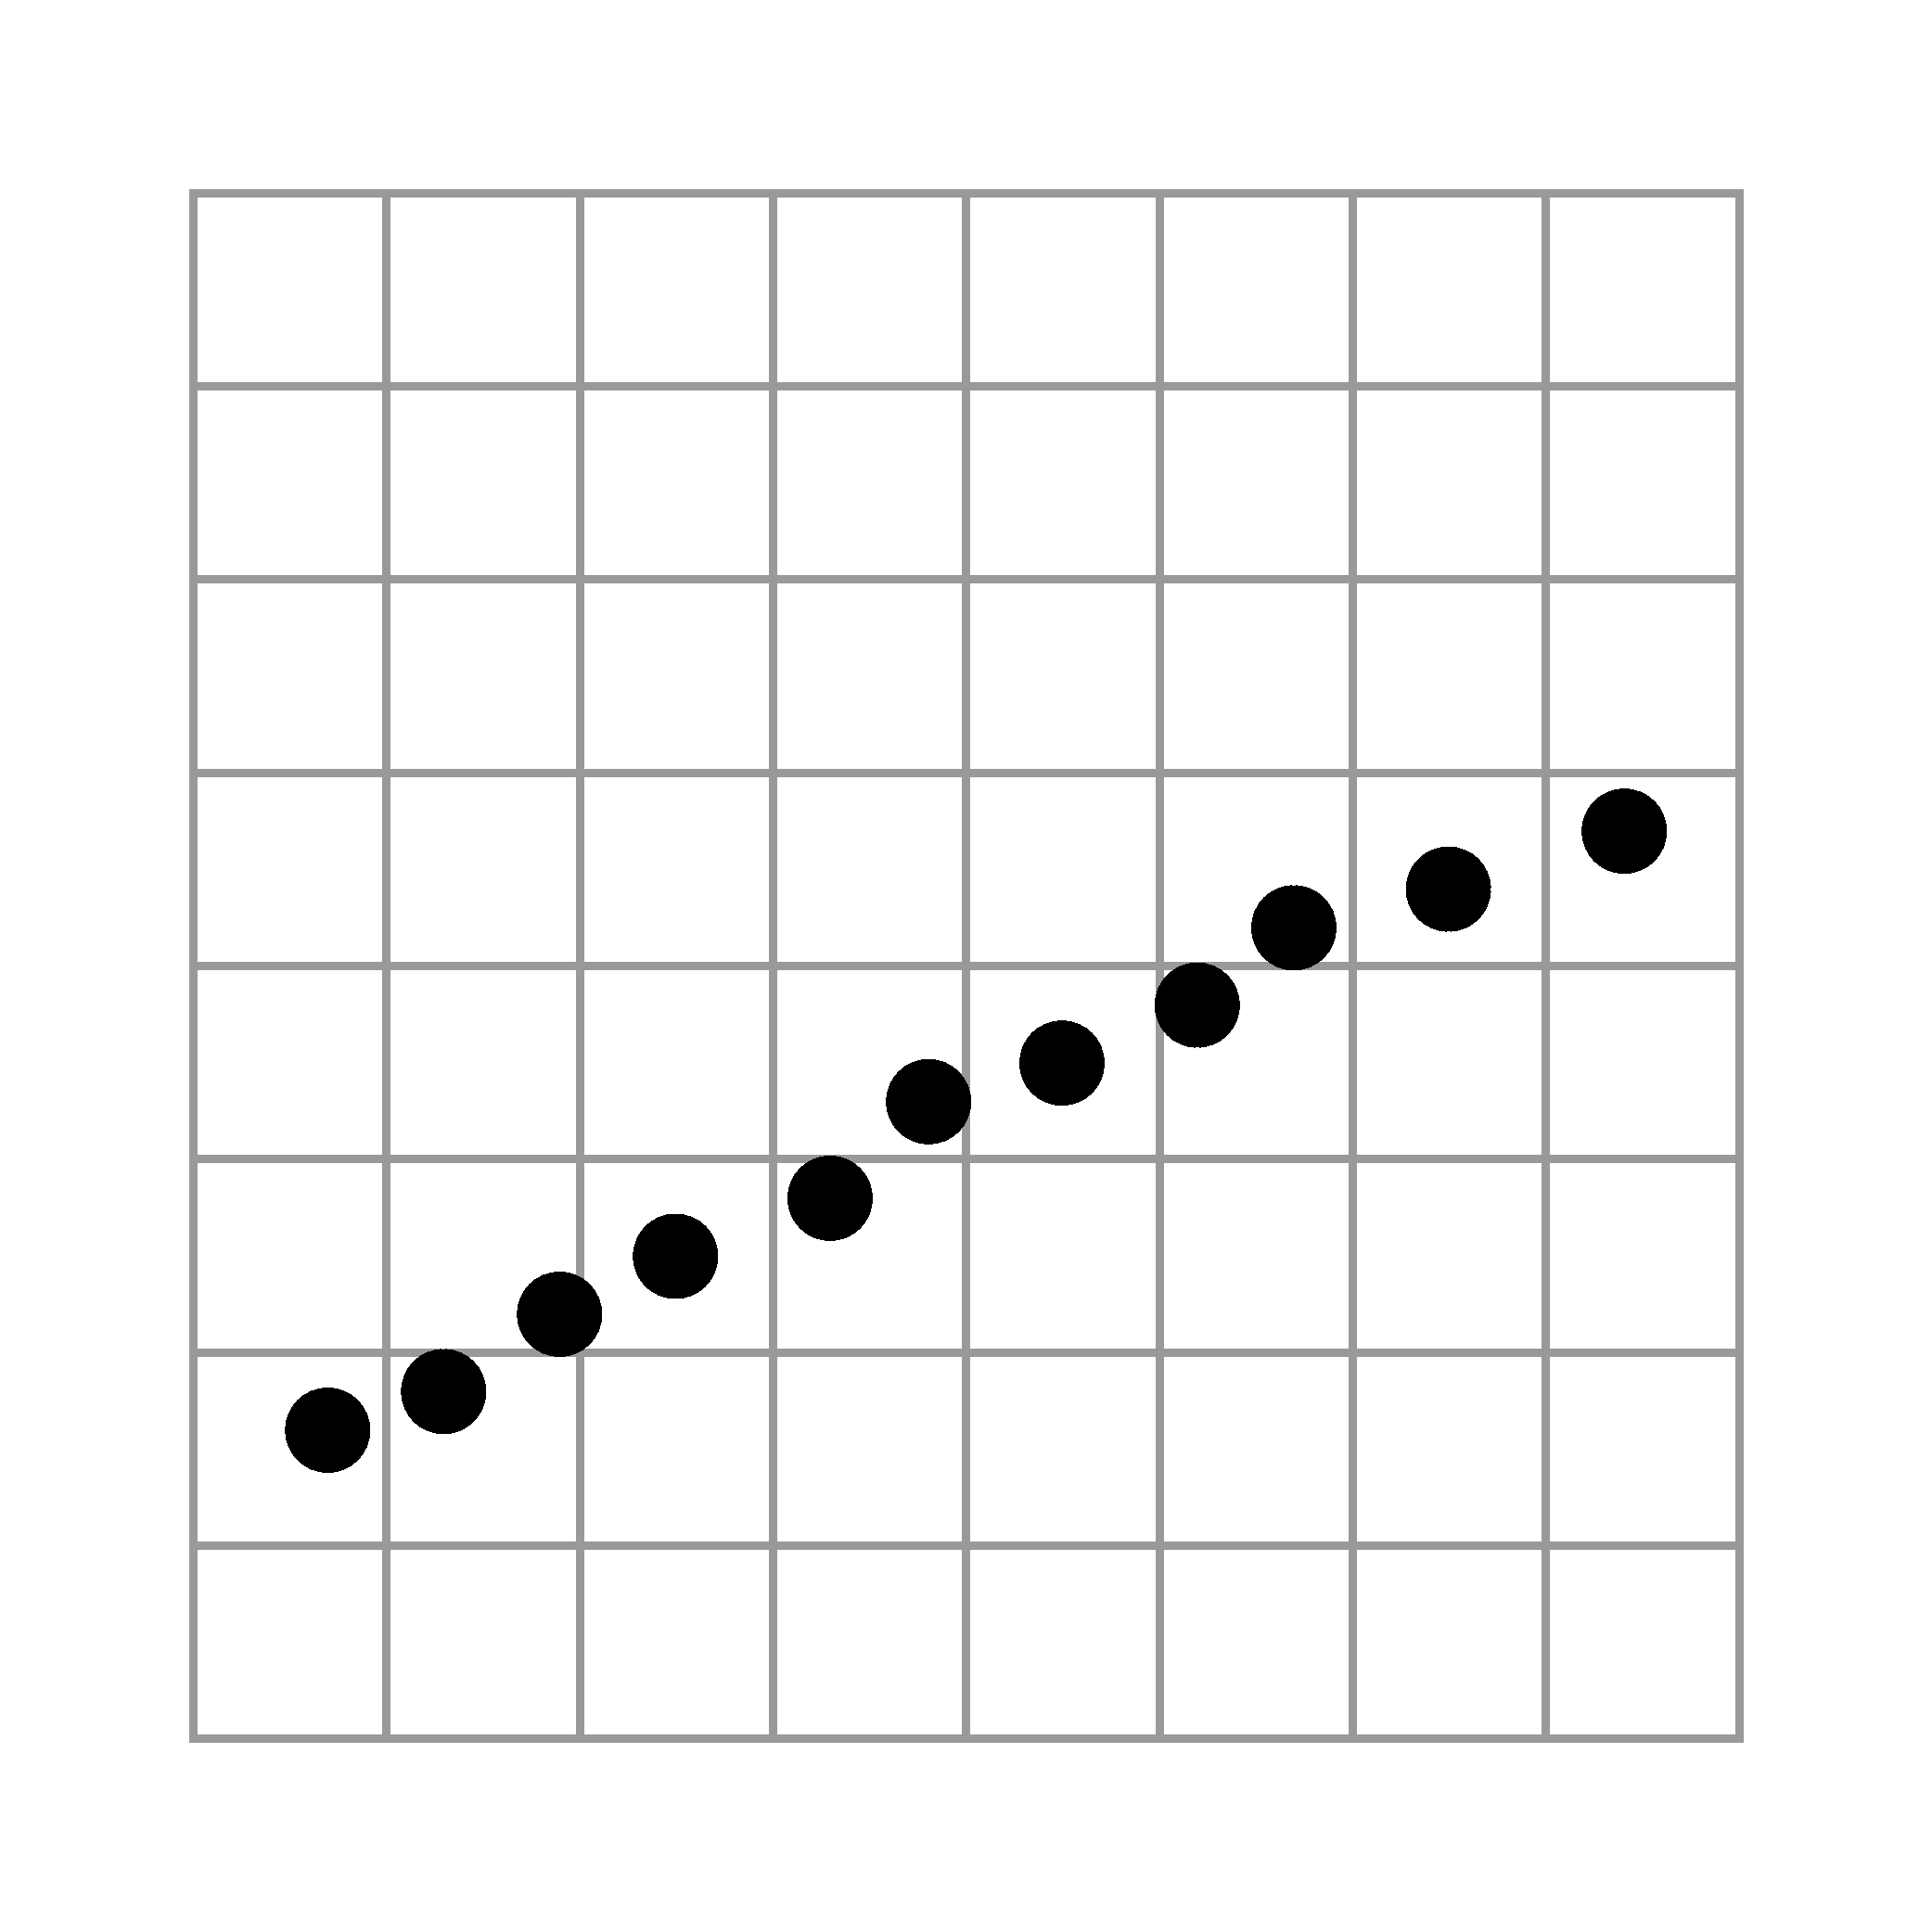
\includegraphics[width=0.4\textwidth]{chapters/cellularautomaton_images/ChargeWeighting2}
	\label{fig:ca_charge_weighting_2}
}
\caption[Diagram of the effect of charge weighting on hit position]{\label{fig:ca_charge_weighting}Schematic diagram of the effect of the charge weighting procedure on hit positions. In \subref{fig:ca_charge_weighting_1} each hit is positioned at the centre of a voxel. In \subref{fig:ca_charge_weighting_2} the hit positions have been adjusted based on the charge-weighted positions of surrounding hits within a $2\mm$ radius; this shifts them from the voxel centres and out of a regular grid structure.}
\end{figure}

\section{Density-based Clustering}
\subsection{\acs{DBSCAN}}\label{sec:latte_dbscan}
The \ac{DBSCAN} algorithm was proposed in 1996 as a means for clustering spatial data based on the varying densities of point clouds\citep{Ester1996}. The algorithm is characterised by its requirement that, for the neighbourhood $\epsilon$ around a given point in the cluster, the number of points $N$ in $\epsilon$ must exceed some threshold value $N_\mathrm{min}$. In this manner, the clustering is determined by identifying areas of high point density. Areas of low point density (i.e. any points not clustered) are identified as \emph{noise} and clustered together as such.

The \ac{DBSCAN} algorithm has been applied to spatial data obtained from a \ac{LAr TPC} by the ArgoNeuT experiment\cite{Spitz2011} to identify clusters in two 2D views, which are subsequently recombined into 3D based on wire readout timing information.

\ac{DBSCAN} has two configurable parameters; $\epsilon$, the radius around a given point within which neighbours must lie, and $N_\mathrm{min}$, the minimum number of those neighbours for a point to be considered part of a dense cluster. While these parameters can be optimised, they remain global, and \ac{DBSCAN} will not typically identify regions of changing density and cluster accordingly. This tends to result in a \ac{DBSCAN} clustering which wraps around the vertex of charged-current neutrino events (for example).

\subsection{\acs{OPTICS}}
The \ac{OPTICS} algorithm\citep{Ankerst1999} extends \ac{DBSCAN} by performing a \emph{hierarchical clustering}; an ordering operation which is equivalent to returning the density-based clusterings associated with a broad range of values of the parameter $\epsilon$. For example, given a fixed value of $N_\mathrm{min}$, clusters obtained with a small $\epsilon$ (that is, high density clusters) are completely contained within the clusters obtained for a larger $\epsilon$ (lower density). \ac{OPTICS} exploits this relationship to provide information about the clustering on all $\epsilon$ scales, allowing clusters to be extracted from spatial data with varying densities.

\section{Feature Detection}\label{sec:latte_feature_detection}
Feature detection refers to the procedure of locating interest points within an image or event. Latte provides two-dimensional feature detection using the method described in \citep{Morgan2010}. Three-dimensional feature detection is currently based on running the two-dimensional feature finder in multiple projections and combining the results.

\subsection{Two-dimensional Feature Detection}
Two-dimensional feature detection uses the \emph{structure tensor} $S$, which is a second-moment matrix defined in terms of the intensity variation of a two-dimensional image:\citep{Morgan2010}
\begin{equation}\label{eqn:structure_tensor}
    S(x,y) = g(\sigma_s) \ast \left[ \begin{array}{cc} I_x(x,y)^2 & I_x(x,y)I_y(x,y) \\ I_x(x,y)I_y(x,y) & I_y(x,y)^2 \end{array} \right]
\end{equation}
where $\ast$ represents convolution, and $I_x(x,y)$ is the partial derivative of the image with respect to $x$ (similarly for $I_y(x,y)$). A Gaussian window $g(\sigma_s)$ is defined as
\begin{equation}\label{eqn:feature_det_gaussian_window}
    g(\sigma) = exp\left( \frac{-(x^2 + y^2)}{2\sigma^2} \right)
\end{equation}
and is used for averaging, as well as noise-reduction.

The eigenvectors and eigenvalues of $S(x,y)$ describe \emph{local} intensity variations within the image. Functions of $S(x,y)$ can therefore be constructed such that their local maxima correspond to features of a desired type. For example, the `V'-like corner of a particle decay vertex will have large intensity changes in all directions. Since it is this type of feature that we are interested in, the F\"orstner-Noble response function $R_N(x,y)$ is used within Latte:
\begin{equation}\label{eqn:forstner-noble}
    R_N(x,y) = \left\{ \begin{array}{cl} \frac{\det S}{\tr S} & \mathrm{if~} \tr S > 0 \\ 0 & \mathrm{if~} \tr S = 0 \end{array} \right.
\end{equation}

This function has local maxima at corner-like features, so the coordinates of these structures correspond to interest points such as decay vertices, interaction points and track endpoints; an example is shown in figure \ref{fig:feature-response}. Note that the feature detection service is used to provide the rough spatial location of a feature that warrants further investigation, and should not be used for precision operations such as vertex fitting.

\begin{figure}
    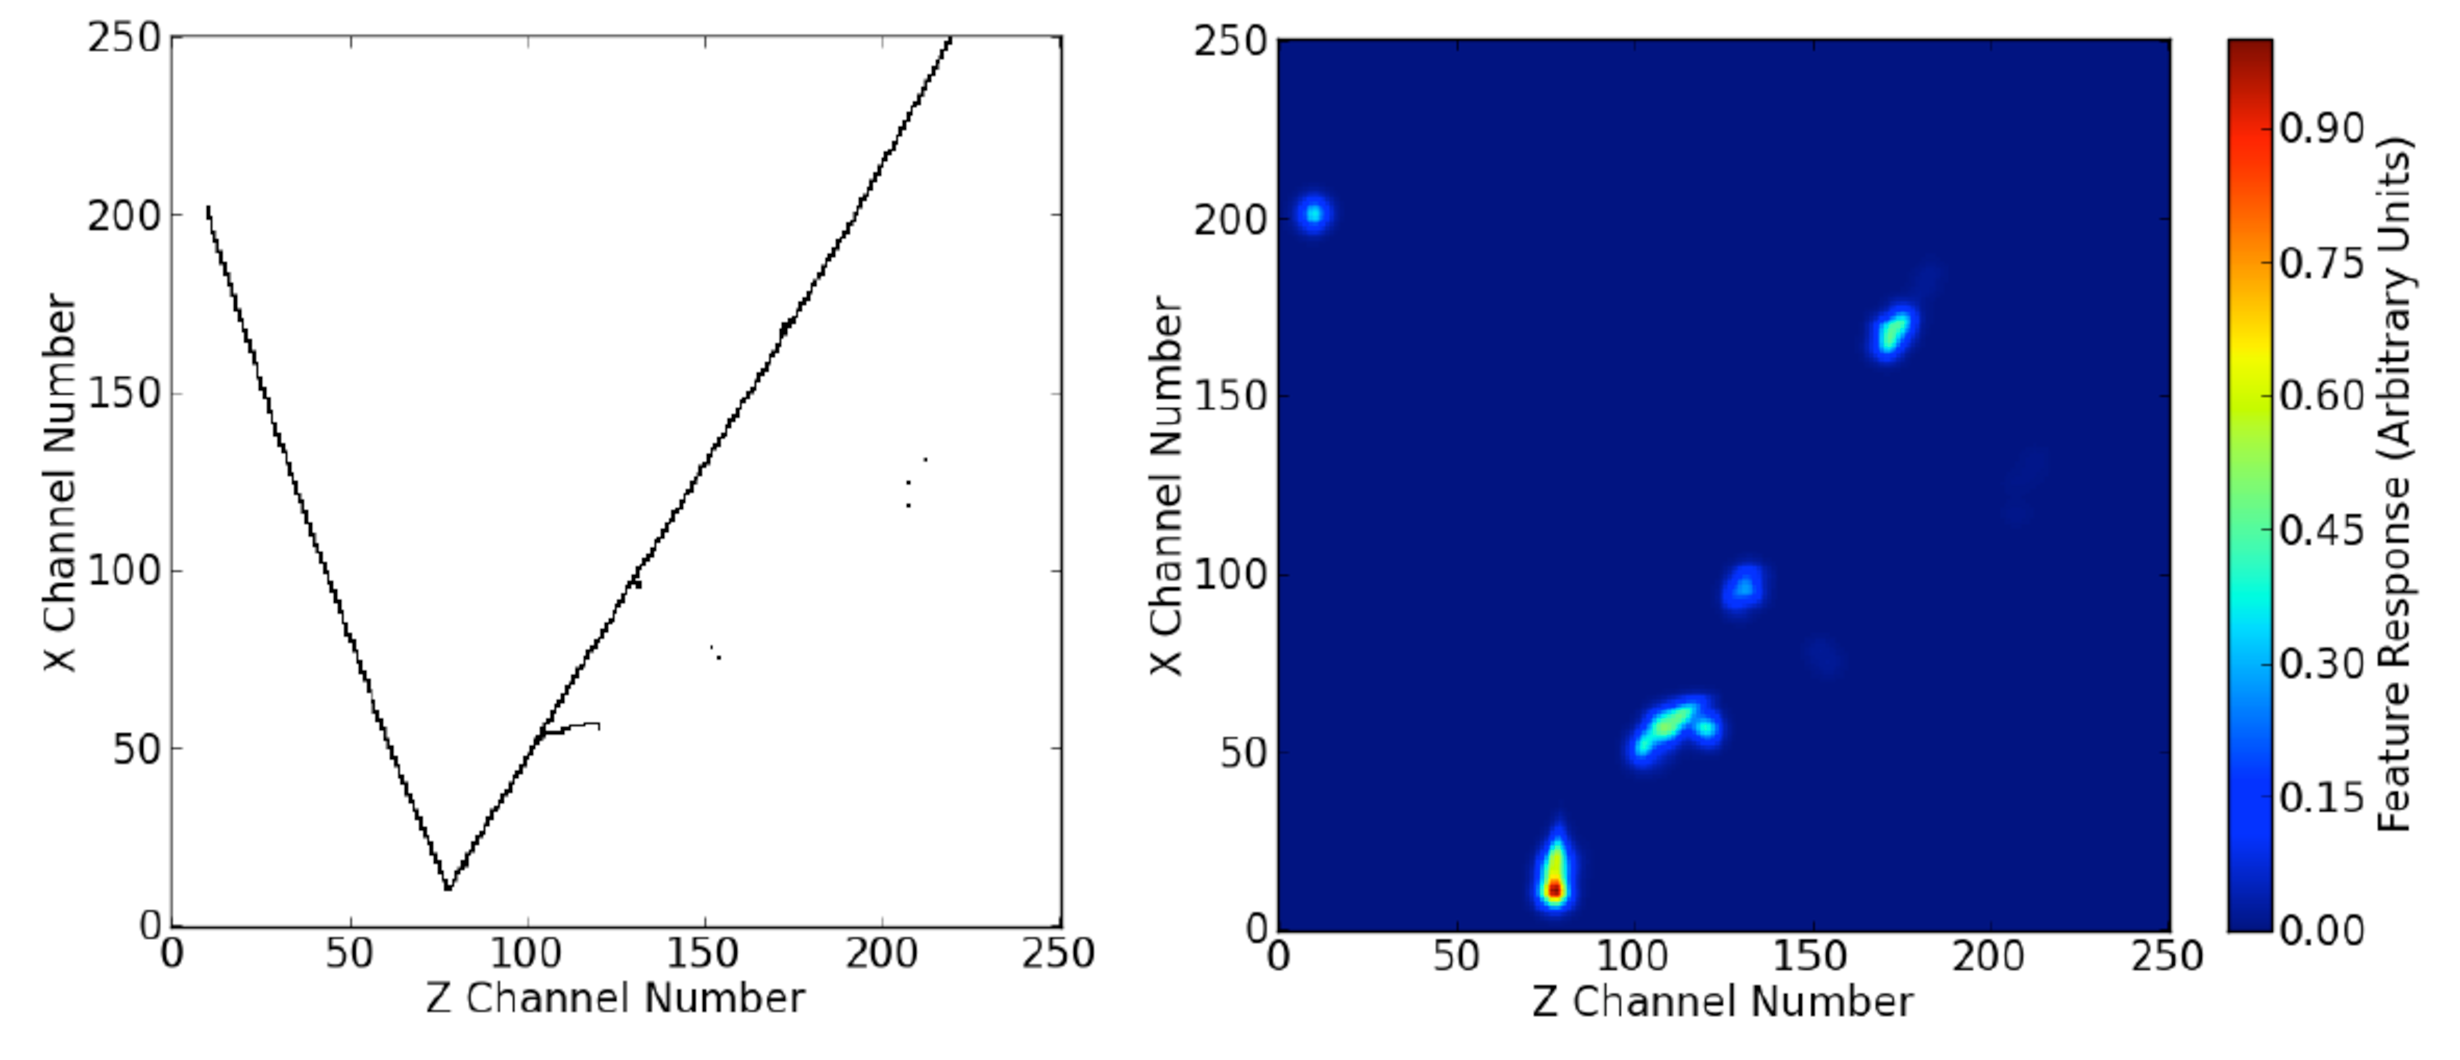
\includegraphics[width=\textwidth]{chapters/latte_images/feature-response}
    \caption[Feature response for a typical neutrino event]{\label{fig:feature-response}A typical neutrino event and the feature response as determined by the feature detection algorithm. The initial vertex and track endpoints are clearly visible, as well as several sites along the right (muon) track where delta electrons were produced.}
\end{figure}

\subsection{Three-dimensional Feature Detection}
Three-dimensional feature detection follows the algorithm outlined below, which uses multiple passes over two-dimensional projections.
\begin{enumerate}
    \item Run 2D feature detection in each of $xy$, $xz$ and $yz$ projections.
    \item Match interest points from each 2D run by requiring a shared coordinate (within some tolerance), e.g. features at $(1,0)$ in $xy$ and $(1,3)$ in $xz$ would be matched.
    \item For each such matching, make a new 3D feature using the information from both points, e.g. for the features above, create a feature at $(1,0,3)$ in $xyz$.
    \item Merge together features in 3D which are within some radial tolerance of each other. This deals with the potential duplicates which may be produced when a feature is visible in all three projections.
    \item Return a list of 3D features which survive the previous steps.
\end{enumerate}

Three-dimensional feature detection implemented in this way is imperfect, since we throw away information from one dimension in each projection, only to recombine the results later. A better approach would be to extend the mathematical definition of the structure tensor, $S$, to 3D (which is trivial) and define a new response function $R_N$ which yields a scalar having large values for corner-like features, and small values elsewhere (which is not trivial).

Despite this limitation, the three-dimensional feature response performs remarkably well. Figure \ref{fig:feature_3d} shows three performance metrics for feature detection applied to 1000 \ac{CCQE} neutrino interactions resulting in a $\mu^{-} + p$ final state. The total number of features found in an event is typically small, with between zero and two features found in most events. For the features found, the displacement from the true interaction vertex is typically small, though this has a long tail all the way to $1000\mm$, which is the radius of the detector used in this simulation. Finally, the normalised response at the true vertex is typically close to $1$, where normalised response is the response at a given feature, divided by the largest response value in the entire event. These characteristics apply even though delta electrons are a large source of noise, having typically high feature response values and appearing throughout the spatial extent of the event.

\begin{figure}
\centering
\subfigure[ ]{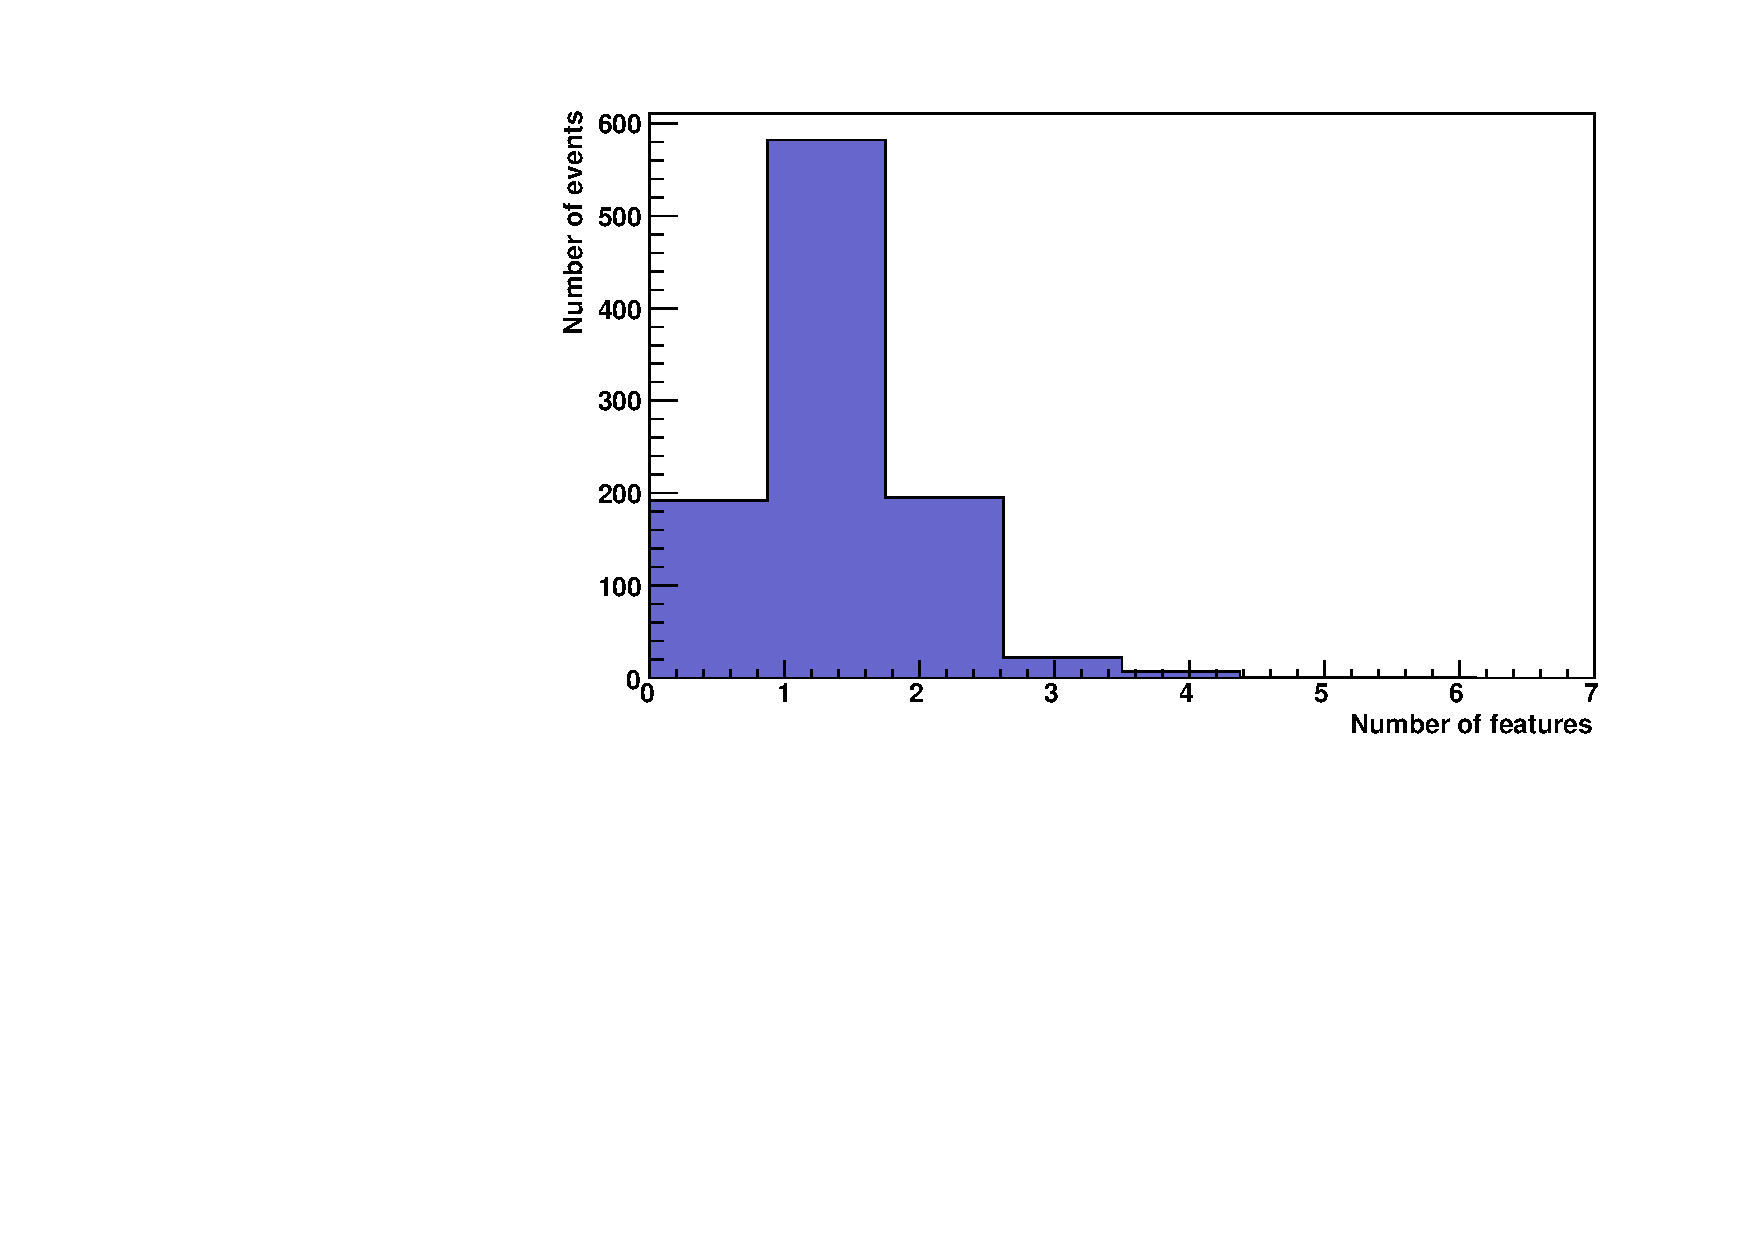
\includegraphics[width=0.35\textwidth,angle=-90]{chapters/latte_images/feature-counts-qel}\label{fig:feature_3d_counts}}
\subfigure[ ]{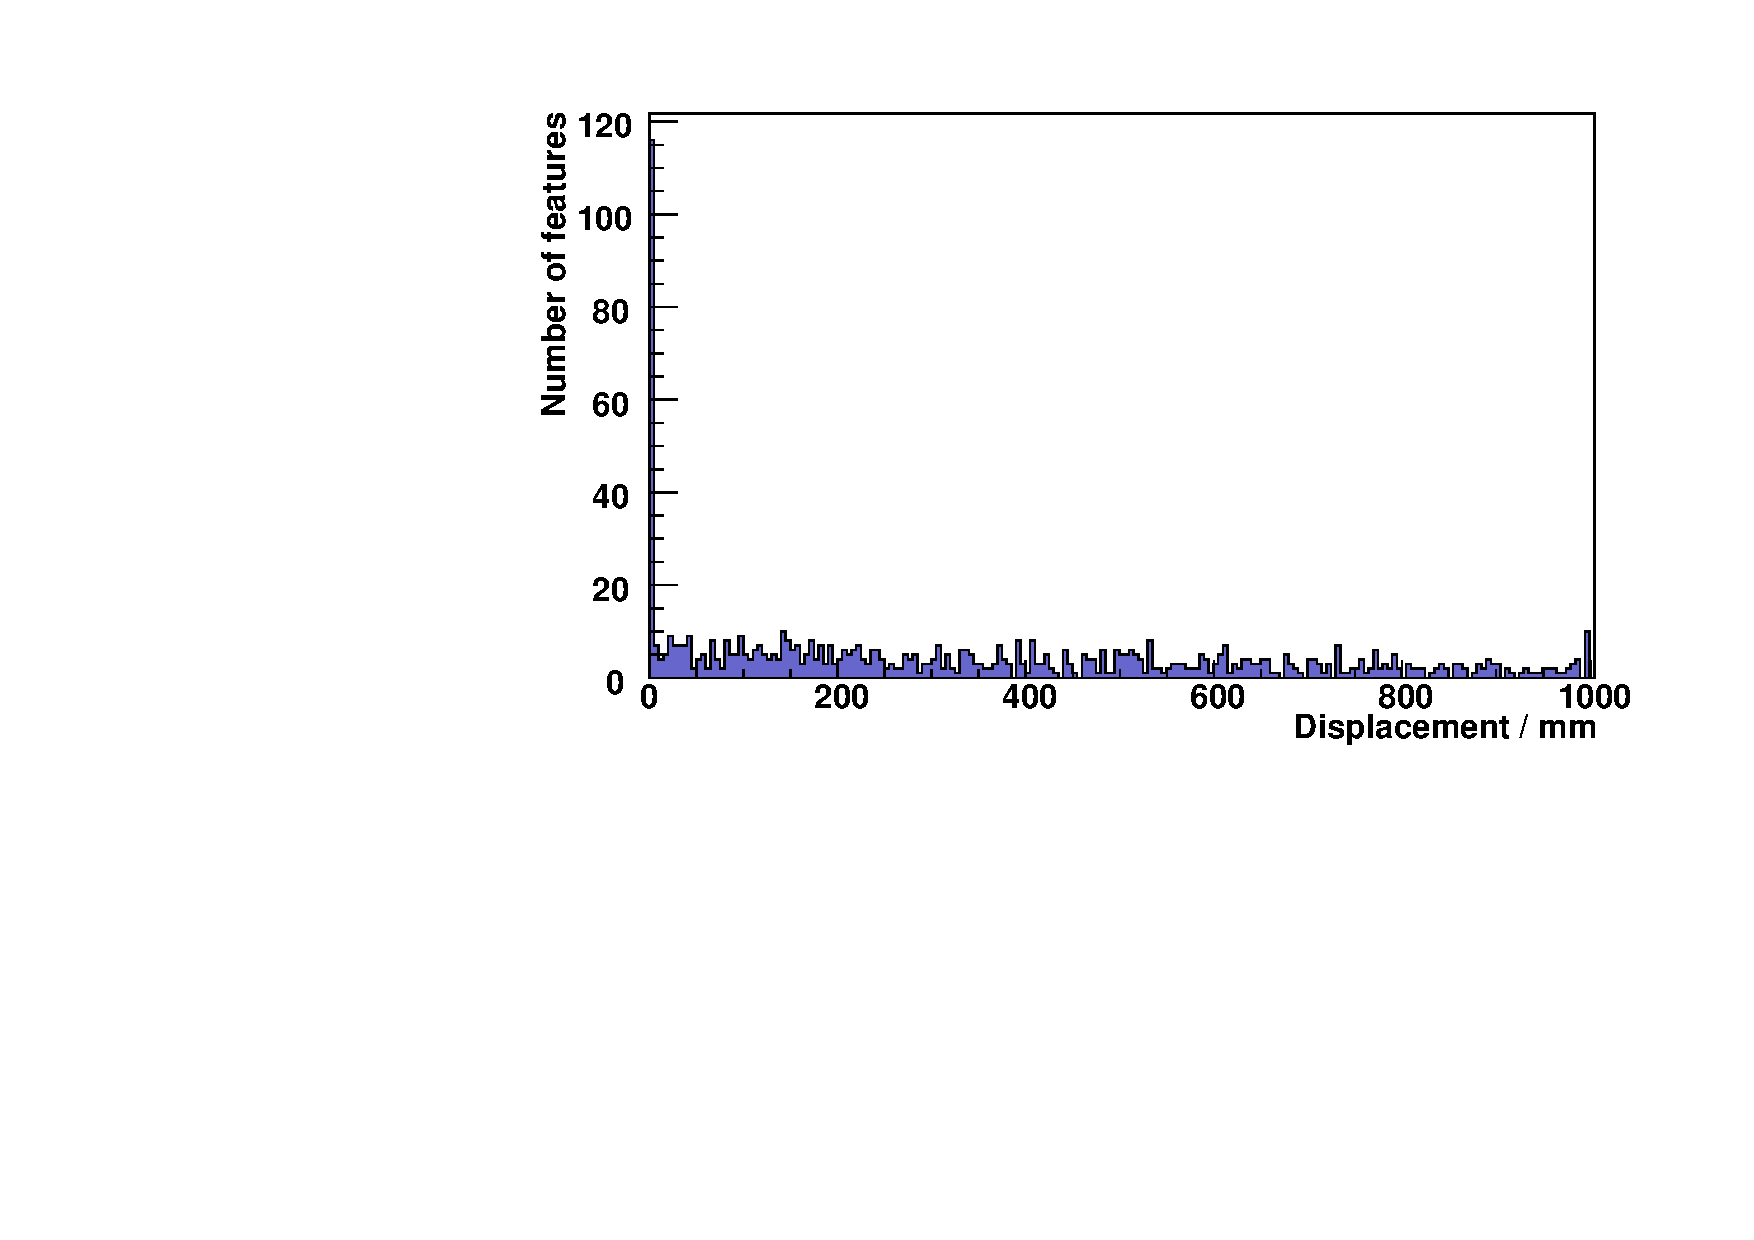
\includegraphics[width=0.35\textwidth,angle=-90]{chapters/latte_images/feature-displacement-qel}\label{fig:feature_3d_displacement}}
\subfigure[ ]{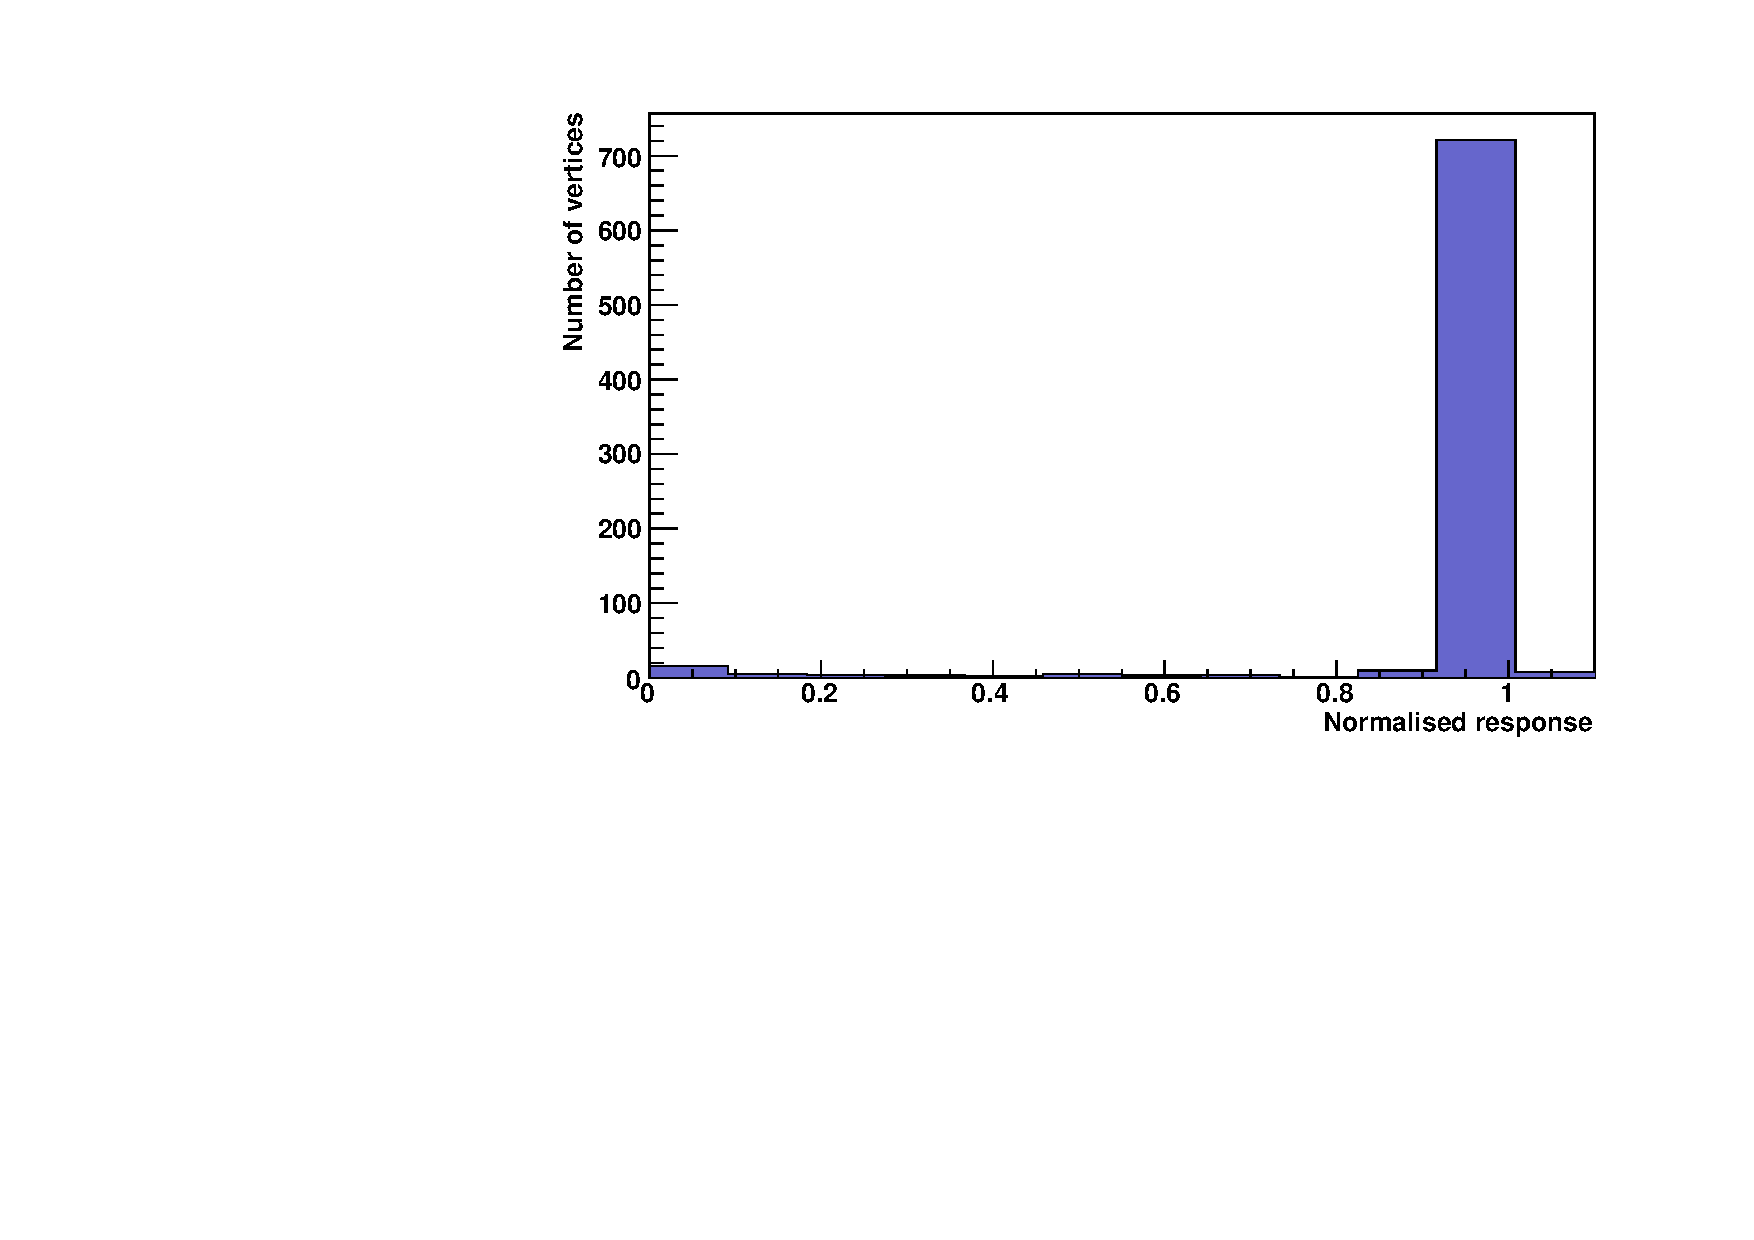
\includegraphics[width=0.35\textwidth,angle=-90]{chapters/latte_images/vertex-feature-response-qel}\label{fig:feature_3d_vertex_response}}
\caption[Performance of the feature detection service in 3D]{\label{fig:feature_3d}Performance of three-dimensional feature detection applied to \acs{CCQE} events. \subref{fig:feature_3d_counts} A small number of features are found in most events. \subref{fig:feature_3d_displacement} The distance between a feature found and the true event vertex is typically small (i.e. features are reasonably well located) but may be anywhere up to the radius of the detector, due to the noise introduced by delta electrons. \subref{fig:feature_3d_vertex_response} The vertex itself typically provides the strongest response of all features in the event.}
\end{figure}

\section{Feature Masking}
Latte provides a service to \emph{mask out} (remove) hits within a spherical region around a feature. The feature masking service presents a new view of the data, which does not include hits positioned less than some radius away from a central point. Each such point can be the location of a feature as determined by the feature detection algorithms of section \ref{sec:latte_feature_detection}, or in a special case the point $(0,0,0)$, referred to as \emph{origin masking}.

This service is useful because it allows algorithms to run on modified views of the event data, which often produces better results. One example would be in a clustering algorithm such as DBSCAN (see \ref{sec:latte_dbscan}), where the local point density affects the clustering. In this case, introducing a gap which corresponds to a feature such as a vertex results in a better clustering of tracks.

\section{Track Merging}\label{sec:cellularautomaton_merging}
Merging is performed using a cylindrical track road algorithm. Track candidates containing more than 100 hits are treated as key tracks for merging. A straight line in 3D is computed for each key track by the procedure below:

\begin{itemize}
	\item Determine a unit vector along the line of the track by using principal components analysis and choosing the component with the largest eigenvalue. This becomes the vector $\vec{n}$ along the line of the track.
	\item Determine a point on the line by computing the centroid coordinate of the hits corresponding to the track. This becomes the vector $\vec{p}$.
\end{itemize}

Each track is then represented by an infinite line in 3D, defined by equation \ref{eq:ca_track_3d_line} where the parameter $\lambda$ is a scalar representing distance along the line from the point $\vec{p}$ at which the point $\vec{l}$ is found.
\begin{equation}\label{eq:ca_track_3d_line}
\vec{l} = \vec{p} + \lambda \vec{n}
\end{equation}

The key tracks are iterated over, beginning with the longest, and hits from other (non-key) tracks are considered for merging into the key track if the distance $d$ from the hit to the line corresponding to the key track is less than some radius $r$. This defines a cylinder of radius $r$ around the key track, inside which any hits from other tracks are merged into the key track. The cylinder extends indefinitely either end of the key track; in practice this is not a problem due to the sparse nature of events resulting from neutrino interactions. Figure \ref{fig:ca_merging_cylinder} illustrates this merging process at a point where a track has been split into two pieces and a third cluster has been identified in the area.

\begin{figure}
\centering
\subfigure[Unmerged tracks]{\label{fig:ca_merging_initial}
	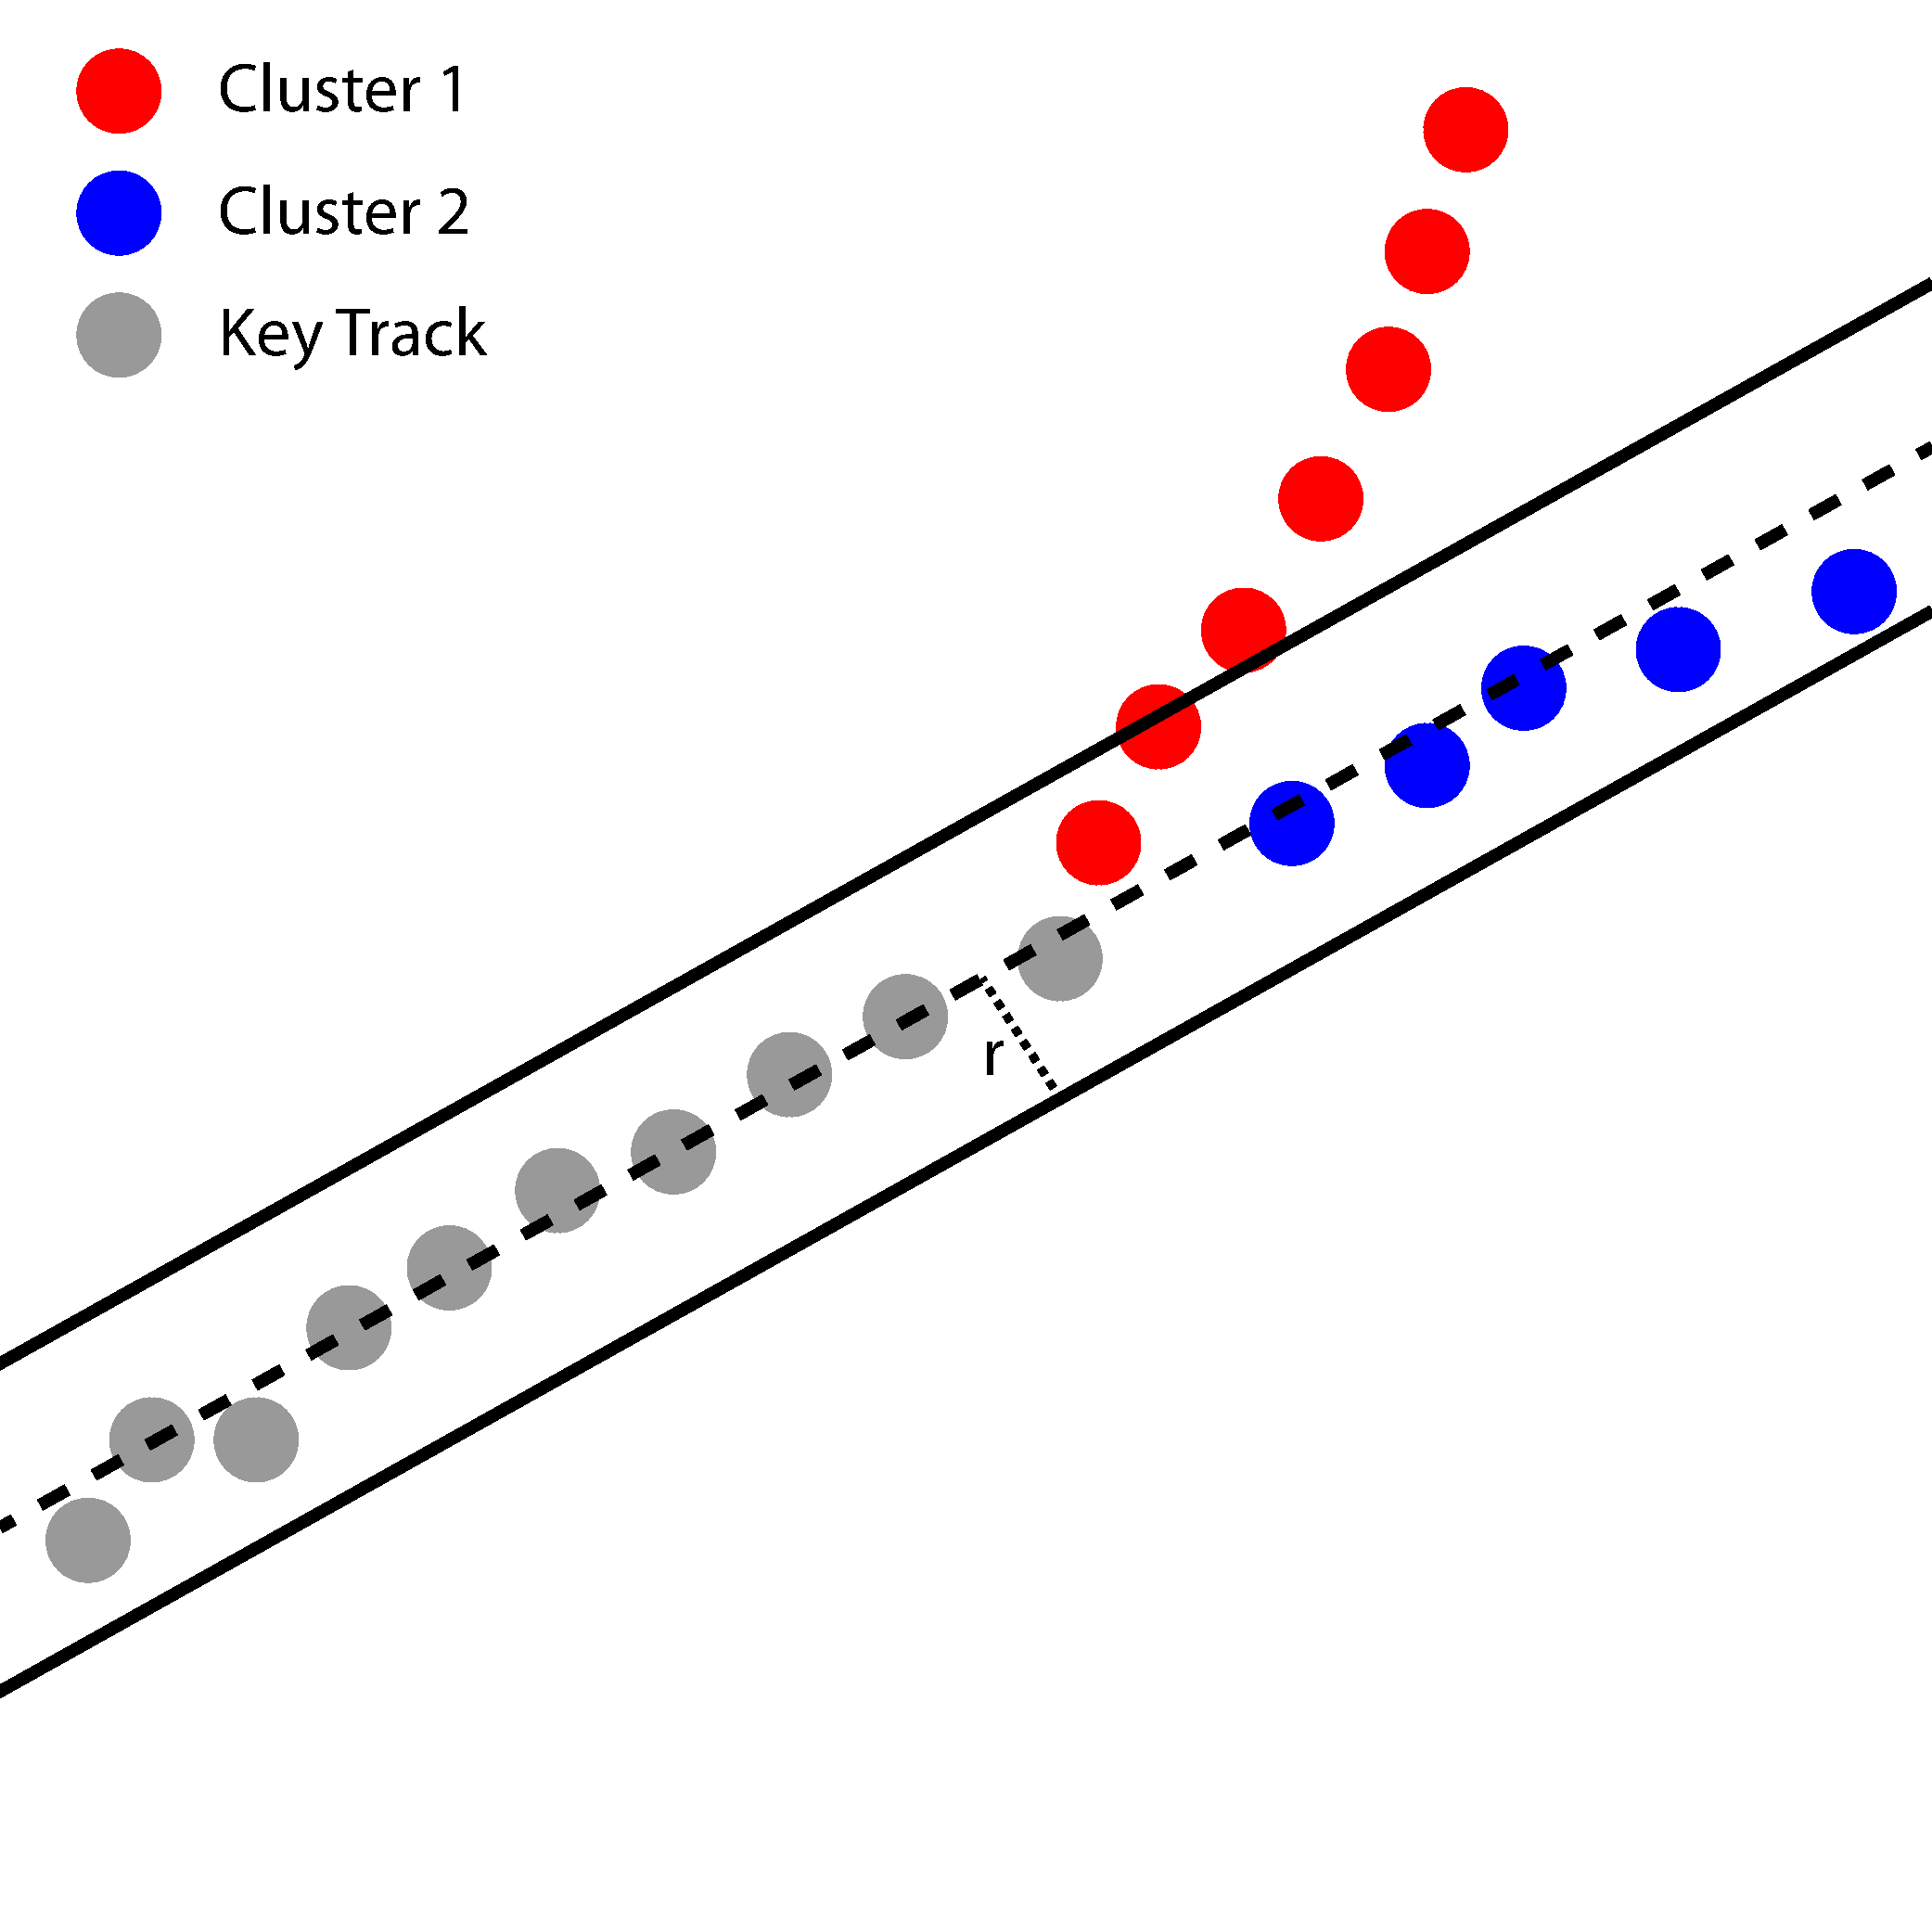
\includegraphics[width=0.35\textwidth]{chapters/cellularautomaton_images/Merging1}
}
\subfigure[Merged tracks]{\label{fig:ca_merging_final}
	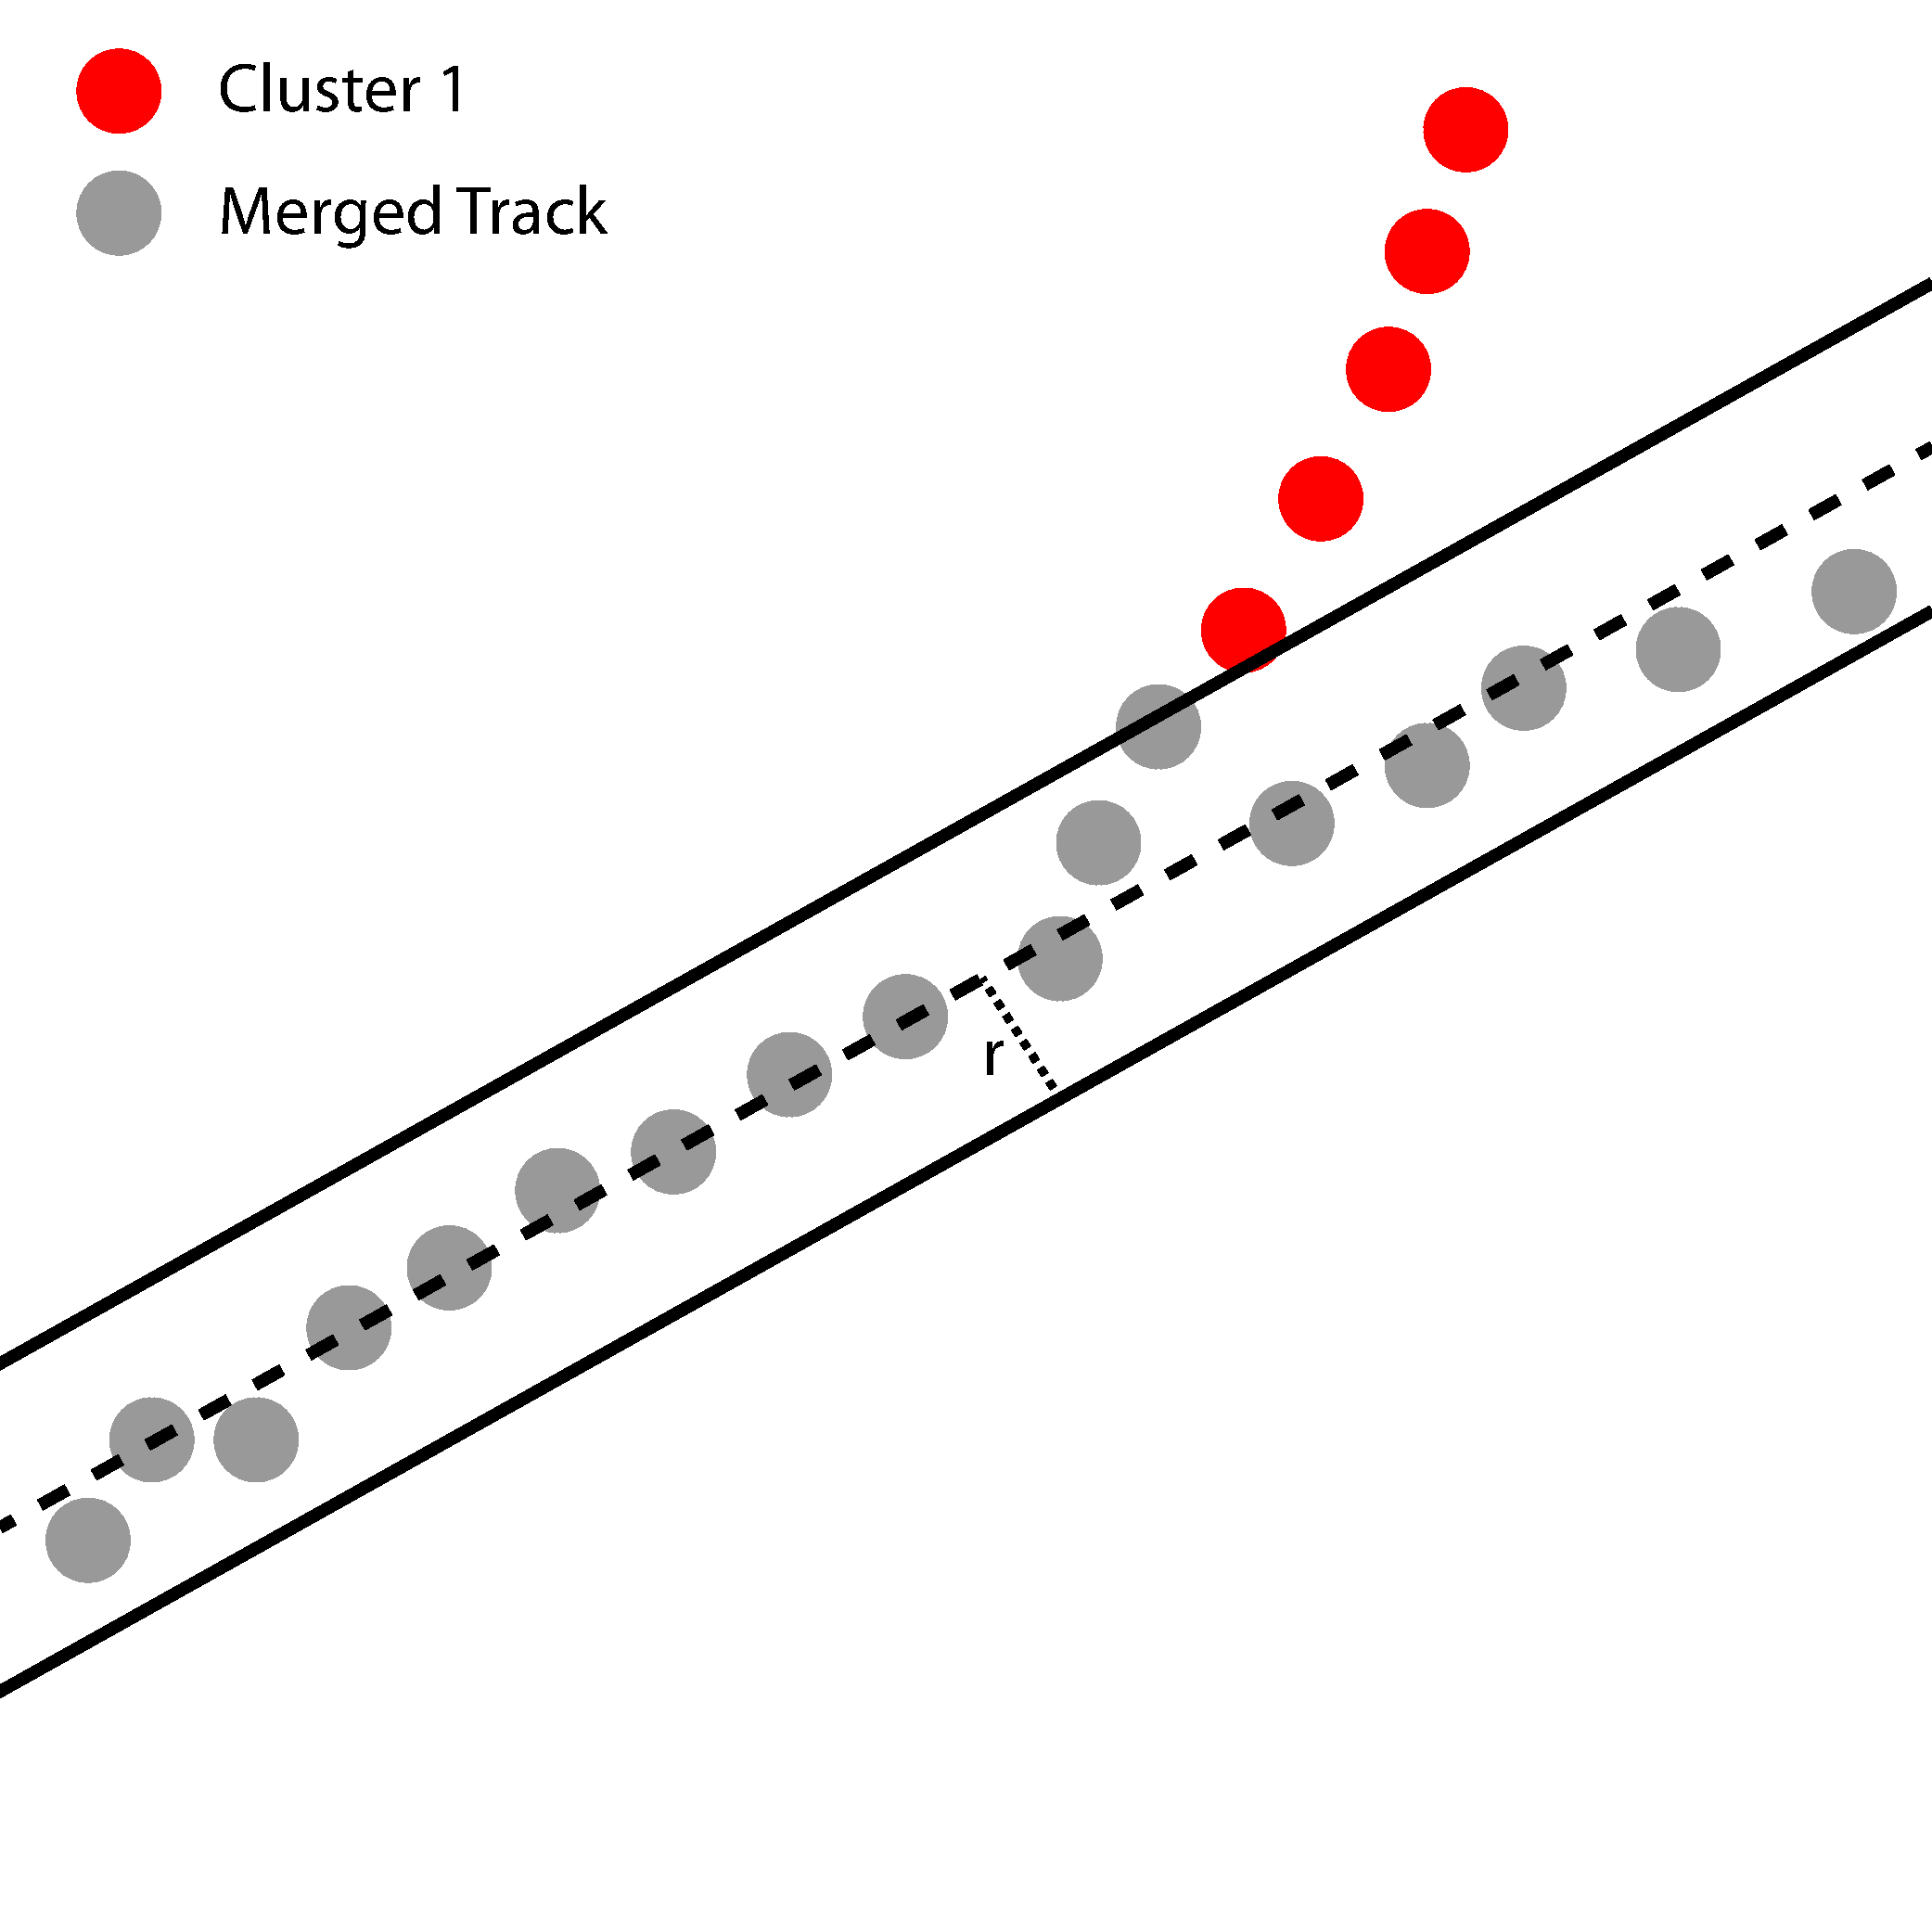
\includegraphics[width=0.35\textwidth]{chapters/cellularautomaton_images/Merging2}
}
\caption[Track road merging algorithm operating on clustered hits]{\label{fig:ca_merging_cylinder}The track road cylinder merging algorithm operating on the output of the \ac{CA}. \subref{fig:ca_merging_initial} shows the initial state with a key track and two smaller clusters. The cylinder drawn around the key track encloses all of cluster 2, but only two hits from cluster 1. \subref{fig:ca_merging_final} shows the resulting merged tracks; hits within the cylinder have been merged such that cluster 2 disappears altogether. Cluster 1 remains but has fewer hits than before.}
\end{figure}

The distance from a hit to the line is defined by taking two points $\vec{x}_1, \vec{x}_2$ on the line (by picking two values of $\lambda$) and, with $\vec{x}_0$ as the coordinates of a hit, the distance is given by equation \ref{eq:ca_dist_hit_line} (see also figure \ref{fig:ca_perp_dist}).
\begin{equation}\label{eq:ca_dist_hit_line}
d = \frac{|(\vec{x}_2 - \vec{x}_1) \times (\vec{x}_1 - \vec{x}_0)|}{|\vec{x}_2 - \vec{x}_1|}
\end{equation}

Hits which are merged into a key track are removed from their original track. Tracks which become empty as a result of this procedure are discarded. This procedure may leave some very small track fragments, which can be cleaned up by applying a range cut requiring any final state track to have some minimum number of hits. Currently, this range cut is set at 20 hits, corresponding to a straight-line track approximately $20\mm$ long, or a minimum ionising particle with $4.2\MeV$ kinetic energy.\footnote{A minimum ionising particle deposits $2.1\MeV \cm^{-1}$ in liquid Argon\citep{Aprile2006}.}

\begin{figure}
\centering
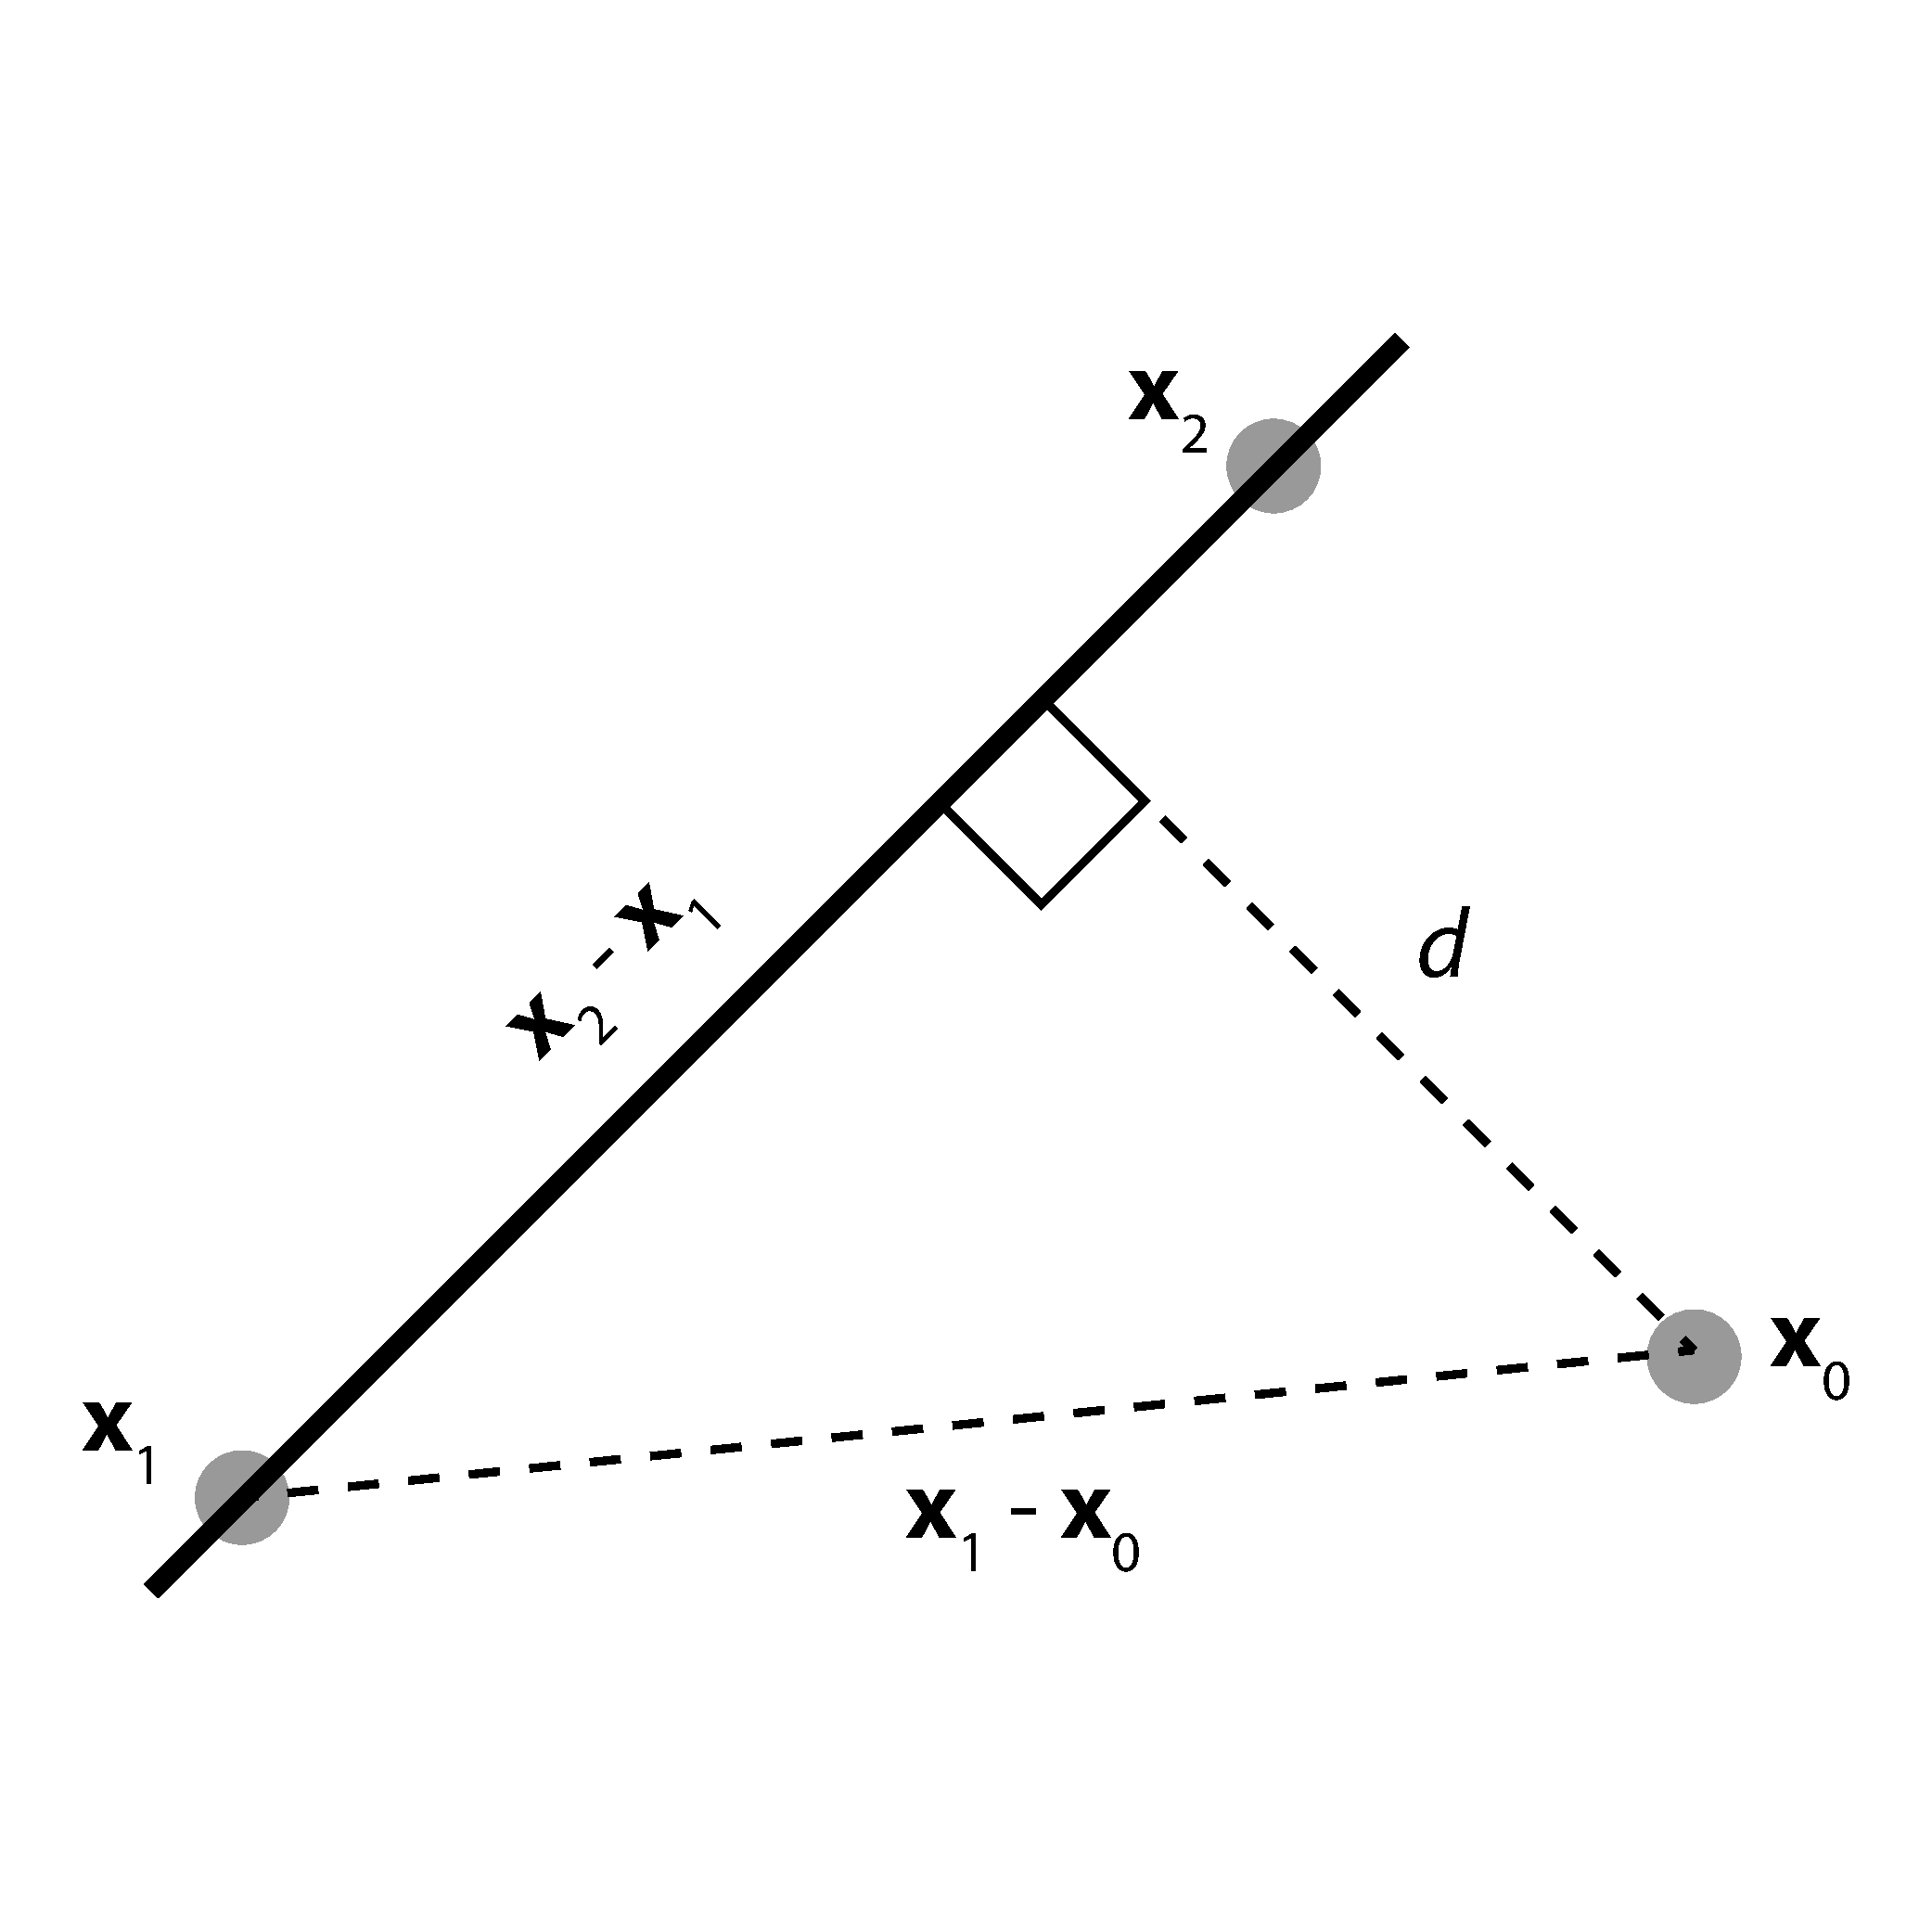
\includegraphics[width=0.5\textwidth]{chapters/cellularautomaton_images/PerpDist}
\caption[Perpendicular distance from a point to a line in 3D]{\label{fig:ca_perp_dist}Illustration of the perpendicular distance $d$ from the point $\vec{x}_0$ to the line between the points $\vec{x}_1$ and $\vec{x}_2$ according to equation \ref{eq:ca_dist_hit_line}.}
\end{figure}


\section{Truth Information}
When working with simulated events, it is often important to be able to access the \emph{truth information}, i.e. the information which was used to generate those events. The Latte framework provides two simulation packages. The first, \emph{PyTrackGen}, generates events consisting of one or more straight line tracks, and is designed to provide simplified representations of common event topologies. The second, \emph{Lamu}, provides a full Geant4 physics simulation, and can be seeded with events from the Genie event generator, or from manually constructed particle sources.

Both kinds of simulation write the truth information corresponding to lines or particles into their output formats, and the Latte framework provides a mechanism to access this information, query it for particle properties, and even make decisions based on it.

It is possible, for instance, to select only hits produced by electrons, or to obtain the true energy of the primary muon from a neutrino interaction. Such quantities are often compared against reconstructed quantities to provide a measure of the success of an algorithm.

\section{Range Cuts}
Latte provides a mechanism to filter event objects based on the number of hits they contain. For track-like objects, this corresponds approximately to the range of the particle. Range cuts can be applied based on the truth information (e.g. to select events where a proton track travelled more than some minimum reconstructible distance), or on reconstructed track objects (e.g. to cut out short track stubs, or to identify long tracks which may correspond to muons).

The range cuts are provided as either filters or wrappers. The filters allow for the selection of events based on track ranges recorded in truth information, while the wrappers present a reduced view of the event, in which the short tracks are not visible.

\section{Latte Control}
Latte Control is a mechanism for applying a sequence of algorithms to a set of events. In its simplest form, it allows the user to set up a \emph{pipeline} composed of service algorithms which are run in sequence on each event stored in a {\sc Root}\citep{Root} file.

\subsection{Event Objects}
A Latte \emph{Event} is essentially a Python dictionary\footnote{A set of key--value pairs. Some languages call them associative arrays, or maps.} with string keys mapped to arbitrary values. The \emph{LamuRun} file reader produces a single key called `raw', which maps to another dictionary containing keys for accessing the raw, simulated data. An \emph{Event object} in Latte Control is a fairly simple wrapper around this plain dictionary.

The wrapper exists primarily to abstract the idea of an event, so that the bulk of the Latte Control framework can deal with the abstract concept of an \emph{event-like object}. An event-like object is any Python object that provides all of the methods in the \texttt{latte.control.event.Event} class. This is useful because it allows us to wrap one event object inside another, thus modifying the behaviour of the event without having to change the original.

The base class, \texttt{latte.control.event.Event}, has the following functionality:
\begin{itemize}
\item A constructor, used internally by event loops (see chapter \ref{sec:latte-event-loops}). This is not usually called by a user of the framework.
\item \texttt{getFilename()}, which retrieves the file from which the event was read.
\item \texttt{getEventID()}, which returns the integer ID of the event within a file.
\item \texttt{getCurrentHitSelection()}, which returns a list of hits.
\item \texttt{getCurrentTracks()}, which returns a list of clusters (tracks).
\item \texttt{getKeys()}, which returns a list of keys defined in the event dictionary.
\item \texttt{hasKey(key)}, which returns \texttt{True} if the key exists, \texttt{False} otherwise.
\item \texttt{setKeyValue(key, value)}, which sets the key \texttt{key} to value \texttt{value}.
\item \texttt{addToKeyValue(key, value)}, which adds \texttt{value} to key \texttt{key}, creating it if it does not already exist.
\item \texttt{getKeyValue(key)}, which retrieves the value associated with the \texttt{key}.
\item \texttt{getUnderlyingEvent()}, which returns the event-like object that this object wraps (or \texttt{self} if it is the innermost layer).
\item \texttt{hasUnderlyingEvent()}, which returns \texttt{True} if this event object wraps another, \texttt{False} otherwise.
\end{itemize}

Most of the methods above allow for access to the keys and values of the dictionary itself. A wrapper class can modify these methods, and by doing so modify the details of how the dictionary is accessed. This allows for great flexibility in defining alternative views of events, for instance, where the set of hits presented differs from the set in the real event (e.g. by application of a range cut, or selection of hits from certain particle types).

In practice, the two most frequently altered methods are \texttt{getCurrentHitSelection()} and \texttt{getCurrentTracks()}. Most algorithms in Latte use these two methods to access the hits or clusters they will work on. In order to provide a modified set of hits or clusters, one simply needs to write an event wrapper to perform the necessary tasks. Event wrappers are discussed in the next section; this is the mechanism by which the range cuts and other modifying services in Latte work, without losing the original event data.

\subsection{Services \& Event Wrappers}
Algorithms made available in the Latte framework can be used with Latte Control in one of two ways. For general purpose reconstruction algorithms, Latte Control provides a corresponding \emph{Service}, which accepts an event object and performs some task. For example, the \emph{Merging} service provides an interface to the track merging algorithms provided in Latte and, when called, runs them on the active track selection. Services usually provide algorithms which are processor-intensive and add new information to the event, for example the allocation of hits to clusters, or the merging of multiple clusters based on certain criteria. Services typically augment an event object with the additional information they are able to provide.

In contrast, there are many cases where the goal of an algorithm is to present a different \emph{view} of the same data. One such example is the charge weighting algorithm, which shifts the position of each hit. Such algorithms are typically brought into the Latte Control framework as \emph{event wrappers}, which intercept attempts to access certain data that are already associated with an event, and present a modified version of that data. In this way, the original data is preserved, and can be retrieved by simply \emph{unwrapping} the event. Each event wrapper provides a \emph{wrapping service} which is used to apply the wrapper at an arbitrary point in the pipeline.

\subsection{Pipelines}
Each event is processed by a \emph{pipeline}, which is simply a sequence of service objects that are called in turn. Some services perform complex tasks such as clustering, while others wrap or unwrap an event, thus changing the views of data available for subsequent services. As events propagate through the pipeline, reconstructed information is added to them by the appropriate services, and may be written to disk (for example) at various points.

Since a Pipeline appears (to an outside observer) as just another callable object which accepts events, it is possible to put pipelines within pipelines, for example to group related services into logical \emph{tasks} (such as grouping clustering and merging of tracks into a \emph{tracking} task), or to provide decision making, using a service which chooses to execute one of several pipelines based on the value (or existence) of certain data in the event.

This flexibility means that the pipeline structure of Latte Control is capable of performing complicated analyses without needing further core support. A user can simply stick together the components they need, in the correct order, then leverage the power of Latte Control to run their analysis job over the available data.

\subsection{Event Loops}\label{sec:latte-event-loops}
At the highest level, Latte Control provides an event loop which is capable of reading a range of events from a {\sc Root} file and passing each event in turn through a pipeline of Latte Control services. In this manner, it is possible to easily write reconstruction scripts which configure a number of services, stick them together in an arbitrary order into a pipeline, and have that pipeline applied to each event in a file. This provides a powerful mechanism for writing physics analysis scripts which make use of the Latte-provided services as well as intermediate or final \emph{analysis} services, using the data available in an event to measure physically useful quantities. Since the objects representing pipeline segments persist between events, they can also be used to build up statistics over an entire set of events. When the event loop finishes, the analysis object can be queried for the set of statistical data it has collected.

